\documentclass{article}
\def\npart {2}
\def\nterm {LMS Summer School}
\def\nyear {2021}
\def\nlecturer {Professor Sarah Whitehouse - University of Sheffield}
\def\ncourse {Combinatorics of Young tableaux and symmetric groups}

\input{header}

\begin{document}
  \maketitle
\ytableausetup{centertableaux}

\section{Overview}

\begin{itemize}
  \item Basic reminders about groups
  \item Definitions of partitions, Young Diagrams and tableaux.
  \item How many standard tableaux are there?
  \item There are two answers; the hook formula and the determinant formula.
  \item Some ideas of the proof - prove the two formulas give the same answer. More detail about the hook formula, via a bijective proof.
  \item Sketch of the relevance to representations of the symmetric group.
\end{itemize}

Useful resource - Bruce E. Sagan, \textit{The Symmetric Group: Representations, Combinatorial Algorithms and Symmetric Functions}

\subsection{Symmetric Group and Permutations}
Let $n \in \N$,

\begin{ndefi}{Symmetric Group}
  The $n^{th}$ symmetric group is $S_n$, and it's the group of all bijections from $\{1, 2, \dots, n\}$ to itself.
\end{ndefi}

Permutations are multiplied from right to left as that's the convention for function composition.\\
There are several standard ways to write perms,
The same permutations $\sigma$ in $S_7$, two line notation,
$$ \begin{matrix}
  1 & 2 & 3 & 4 & 5 & 6 & 7 \\
  6 & 2 & 5 & 7 & 3 & 4 & 1
\end{matrix} $$
and one line notation,
$$ \begin{matrix}
  6 & 2 & 5 & 7 & 3 & 4 & 1
\end{matrix} $$
and in cycle notation,
$ (1 6 4 7)(3 5)(2) $ or $ (1 6 4 7)(3 5) $
this means that $1 \to 6 \to 4 \to 7 \to 1 \dots$ and $3 \to 5 \to 3 \to \dots$ and $2$ maps to itself. The two doesn't necessarily need to be written as it may be seen as redundant.\\

The composition of $\pi\sigma$ where $\sigma = (1 6 4 7)(3 5)(2) $ and $\pi = (1 4)$, then,
$$ \pi\sigma = (1 4)(1 6 4 7)(3 5) = (1 6)(3 5)(4 7) $$
this isn't very efficient as there are things written more than once. Read right to left, and just work through it and write it down.

\begin{ndefi}{k-cycle}
  A $K$-cycle is a cycle containing k elements
\end{ndefi}
The cycle type of a permutation is an expression of the form $(1^{m_1}, 2^{m_2}, \dots, n^{m_n})$ where $M_k$ is the number of k-cycles.\\
For example, $\sigma$ has cycle type, $(1^1, 2^1, 3^0, 4^1, 5^0, 6^0, 7^0)$.\\

\begin{ndefi}{Conjugation}
  In Group Theory, take a group $G$, the elements $g$ and $h$ are conjugate if the exists some $k\in G$, st, $g = khk^{-1}$.
\end{ndefi}
Conjugacity is an equivalence relation, so the group splits up into non-intersecting conjugacy classes.\\
\begin{ndefi}{Conjugacy Class}
  The set of all elements conjugate to $g \in G$ is called the conjugacy class of $g$.
\end{ndefi}

\subparagraph{Conjugacy Classes and Cycle Types}
\begin{remark}
  For the inverse, write down each of the elements in reverse order.
\end{remark}

If,
$$ \pi = (i_1, i_2, \dots, i_l)\dots (i_r, i_{r+1}, \dots, i_n) \in S_n $$
then,
$$ \sigma\pi\sigma^{-1} = (\sigma(i_1), \sigma(i_2), \dots, \sigma(i_l))\dots (\sigma(i_r), \sigma(i_{r+1}), \dots, \sigma(i_n)) $$
You have the same cycle type, you just `apply' $\sigma$. Same cycle type and the number replaced with what you are conjugating by. For example, $\pi = (1 4)$ (2 cycle, transposition) and $\sigma = (1 6 4 7)(3 5)$ as before, $\sigma \pi \sigma^{-1} = (6 7) $. It follows that,
\begin{nlemma}
  Two permutations are conjugate if and only if they have the same cycle type.
\end{nlemma}
We haven't only done one side as if we take a $\sigma$, we can just take an appropriate $\pi$.\\

Conjugacy is very important in group theory, they are used in classification results and philoe theorems. A group acts on itself by conjugation, it acts by conjugation of that group action. You have orbits and stabilizers and you can deduce things about the structure of the group. There are irreducible representations and there is each one for each conjugacy class of the group.

\section{Paritions and Young Tableaux}

\begin{ndefi}{\textit{Partition}}
  A partition of $n$ is a finite sequence of natural numbers $\l = (\l_1, \l_2, \dots, \l_r)$ where $\l_i \ge \l_{i+1}$ for all $i$ and $\sum_{i=1}^r \l_i = n$. We write $(\l_1, \l_2, \dots, \l_r) \vdash n$ this to mean partition,
\end{ndefi}

For example, $(5, 3, 1) \vdash 9$. We represent paritions by diagrams, in the form of left justified arrays of boxes. For the partition $(\l_1, \l_2, \dots, \l_r)$, we draw $\l_1$ on the top, then $\l_2$, and so on. Let us take $(5, 3, 1)$.

We saw earlier that two elements of $S_n$ are in the same conjugacy class if and only if they have the same cycle type.\\
We can equivalent record a cycle by a partition of $n$. For our previous example, $\s = (1 6 4 7)(3 5)(2)$ and record the cycle type as $(4, 2, 1)$, as per our pervious definition. This means that there are a bijection between partitions of $n$ \\

\begin{figure}[!ht]
  \centering
  \ydiagram{5,3, 1}
  \caption{A Young Diagram}
  % \label{}
\end{figure}

\begin{ndefi}
  A Young Tableau of shape $\l$, where $\l \vdash n$, is a bijective assignment of the numbers $1, 2, \dots, n$  to the boxes of the diagram of $\l$.
\end{ndefi}

\begin{figure}[!ht]
  \centering
  \begin{ytableau}
         4 & 1 & 7 & 3 & 6 & 2 \\
         1 & \none
  \end{ytableau}
  \caption{A Youngs Tableau}
\end{figure}

% add Young Tableaux

Clearly, the number of such tableaux is $n!$. Such a tableaux is called standard if each column and row is increasing.\\
First we fix $n$, then draw the diagram and then assign $1$ up to $n$ into the boxes with constraints of increasing in each row and column. We will write $f^\l$ as the number of standard young tableaux of shape $\l$. Understanding the number of $f^\l$ and our importance will be our focus.

\subsection{Alfred Young}
Reverend Alphred Young, came up with the tableaux. ``The original man of the year, who would have ranked a higher place in the list had he directed his attention to the examination schedule''. He attaned a 2:2 from Cambridge.

\subsection{Tableaux}
We are going to consider $S_3$. Here are the 6 young tableaux of shape $(2, 1)$.
\begin{figure}[!ht]
  \centering
  \begin{ytableau}
         1 & 2 \\
         3 & \none
  \end{ytableau}
  \begin{ytableau}
         1 & 3 \\
         2 & \none
  \end{ytableau}
  \begin{ytableau}
         2 & 3 \\
         1 & \none
  \end{ytableau}
  \begin{ytableau}
         2 & 1 \\
         3 & \none
  \end{ytableau}
  \begin{ytableau}
         3 & 1 \\
         2 & \none
  \end{ytableau}
  \begin{ytableau}
         3 & 2 \\
         1 & \none
  \end{ytableau}
  \caption{The Young Tableaux for $(2, 1)$.}
  % \label{}
\end{figure}



% write out each of the diagrams.
The first two are standard tableaux and the rest are not. The conclusion is that $f^{(2, 1)} = 2$.

\section{Hook and Determinant Formula}
\subsection{Hook Formula}

The box in row $i$ and column $j$ has coordinate $(i, j)$. For example this is $(2, 3)$

% add diagram

Let $\l \vdash n$. For the box $b$ with coordinates $(i, j)$ in the diagram of the shape $\l$, its hook, $H_b$ consists of all the boxes in the same row from $b$ onwards and the boxes from $b$ downwards.

$$ H_n \{(i, j') \text{ a box of } \l \,|\, j' \ge j\} \cup \{(i', j) \text{ a box of } \l \,|\, i' \ge i\} $$

For example, the hook of $(1, 2)$ is shown,

\begin{figure}[!ht]
  \centering
  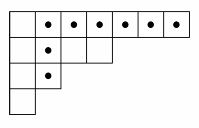
\includegraphics{./figures/L2.1}
  \caption{}
  % \label{}
\end{figure}

The corresponding hooklength, $h_b = h_{i, j}$ is the number of boxes in the hook:
$$ h_b = |H_b| $$
each box has a hook length.
\begin{figure}[!ht]
  \centering
  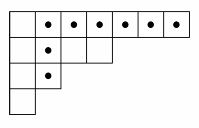
\includegraphics{./figures/L2.1}
  \caption{}
  % \label{}
\end{figure}
In the example $h_{1, 2} = 8$.

\begin{nthm}
  For $\l \vdash n$,
  $$ f^\l = \frac{n!}{\prod_{(i, j) \in \l} h_{i,j}} $$
\end{nthm}

For $\l = (3, 2) \vdash 5$, the hook lengths are indicated for each box.

\begin{figure}[!ht]
  \centering
  \begin{ytableau}
         4 & 3 & 1 \\
         2 & 1 & \none
  \end{ytableau}
\end{figure}
and the hook formula gives us that,
$$ f^{(3, 2)} = \frac{5!}{4 \cdot 3 \cdot 2} = 5 $$
\newpage
Now consider this diagram, again same numbering convention,
\begin{figure}[!ht]
  \centering
  \begin{ytableau}
         9 & 7 & 6 & 4 & 2 & 1 \\
         6 & 4 & 3 & 1 & \none & \none\\
         4 & 2 & 1 & \none & \none & \none\\
         1 & \none & \none & \none & \none & \none\\
  \end{ytableau}
\end{figure}

and the formula gives, $f^{(6, 4, 3, 1)} = \frac{14!}{9 \cdot 7 \cdot 6 \cdot 4 \cdot 2 \cdot 6 \cdot 4 \cdot 3 \cdot 4 \cdot 2}$


\subsection{Determinant Formula}
Let's look at another formula for $f^\l$ calculated via a determinant.\\

We will use the convention that $\frac{1}{r!} = 0$ if $r < 0$ and $0! = 1$.

\begin{nthm}
  For $\l = (\l_1, \l_2, \dots, \l_r) \vdash n$,
  $$ f^\l = n! \left| \frac{1}{(\l_i-i+j)!} \right| $$
  where the determinant is of an $r \times r$ matrix (the thing in the mod symbols is what the matrix is defined as, i.e. $a_{ij} = \frac{1}{(\l_i-i+j)!}$).
\end{nthm}

For $\l = (3, 2) \vdash 5$, we get,
$$ f^{(3, 2)} = 5! \left|\begin{matrix}
  \frac{1}{3!} & \frac{1}{4!}\\
  \frac{1}{1!} & \frac{1}{2!}
\end{matrix}\right| $$
and we can calculate this,
\begin{align*}
  f^\l &= 5! (\frac{1}{6} \cdot \frac{1}{2} - \frac{1}{24})\\
  &= 5!\left(\frac{1}{24}\right)\\
  &= 5
\end{align*}

\begin{remark}
  To write down the correct denominators in the determinant, note that the factorials of the parts of $\l$ appear down the main diagonal. The other entries involve increasing the number in the factorial by $1$ for each step to the right and decrease it by one to the left.
\end{remark}

For $\l = (4, 2, 2, 1) \vdash 9$, we get,
$$ f^{(4, 2, 2, 1)} = 9!\left| \begin{matrix}
  \frac{1}{4!} & \frac{1}{5!} & \frac{1}{6!} & \frac{1}{7!}\\
  \frac{1}{1!} & \frac{1}{2!} & \frac{1}{3!} & \frac{1}{4!}\\
  \frac{1}{0!} & \frac{1}{1!} & \frac{1}{2!} & \frac{1}{3!}\\
  0 & 0 & \frac{1}{0!} & \frac{1}{1!}\\
  % more here
\end{matrix} \right|  $$

\subsection{Proving Equality}

Now we aim to assertain that for $\l = (\l_1, \dots, \l_r) \vdash n$,
$$ \frac{n!}{\prod_{(i, j) \in \l}h_{i, j}} = n! \left| \frac{1}{(\l_i-i+j)!} \right| $$
Equivalently,
$$ \frac{1}{\prod_{(i, j) \in \l}h_{i, j}} = \left| \frac{1}{(\l_i-i+j)!} \right| $$

We are going to write $\det_\l$ for the determinant on the right hand side. The first thing to do is to write $\det_\l$ in terms of hook lengths of boxes in the first column of the diagram of $\l$, using,
$$ \l_i - i + r = h_{i,1} $$
\begin{ex}
  This is an exercise, draw a diagram. If a partition has $r$ parts, it has $r$ rows in the diagram.
\end{ex}
So,
$$ \det_\l = \left| \frac{1}{(h_{i,1} - r + j)!} \right| $$
Now we are going to do induction on $n$. The main step is removing the first column and comparing. So check some base case, for $n = 1$. Since $\l = (1)$ and,
$$ \det_{(1)} = 1 = \frac{1}{h_{1,1}} $$

Lets write $\overline{\l}$ for the partition corresponding to removing the first column of the diagram $\l$. So,
$$ \overline{\l} =(\l_1 - 1, \l_2 - 1, \dots, \l_3 - 1) $$
($\overline{\l}$ could have less entries than $\l$).
\begin{figure}[!ht]
  \centering
  \ydiagram{6,4, 2}
  \caption{ $\l = (6, 4, 2)$}
\end{figure}
\begin{figure}[!ht]
  \centering
  \ydiagram{5,3,1}
  \caption{ $\overline{\l} = (5, 3, 1)$}
\end{figure}

Notice that the hook length of $\overline{\l}$ are the hook lengths $h_{i,j}$ of $\l$, for $j \ge 2$, that is excluding those for boxes in the first column. Use row and column operations to show that,
$$ \det_\l = \prod_{i=1}^r \frac{1}{h_{i, 1}}\det_{\overline{\l}} $$
The result then follows by induction. \\
A bit of care is needed in the case where $\overline{\l}$ has fewer rows than $\l$, but it still works. This relates to the conventions we made, but it still works out OK.

\subsubsection{Row and Column Operations}
Lets write $C_j$ for the $j^{th}$ column.
\begin{itemize}
  \item Pull out $\frac{1}{h_{i, 1}!}$ from row $i$ for each $i$
  \item Replace $C_1$ by $C_2 - C_1$ % could be wrong
  \item Replace $C_2$ by $C_3 - 2C_2$
  \item Continue in this way, replacing $C_{j-1}$ by $C_j - (j - 1)C_{j-1}$ for $4 \le j \le r$
  \item Put  $\frac{1}{h_{i, 1}!}$ back into row $i$.
\end{itemize}

Let's consider $\l = (3, 2) \vdash 5$,
\begin{figure}[!ht]
  \centering
  \begin{ytableau}
         4 & 3 & 1 \\
         2 & 1 & \none
  \end{ytableau}
\end{figure}

So we have $h_{1, 1} = 4$, $h_{2, 1} = 2$. Removing the first column gives $\overline{\l} = (2, 1) \vdash 3$.

\begin{align*}
  \det_{3, 2} &= \left| \begin{matrix}
    \frac{1}{3!} & \frac{1}{4!}\\
    \frac{1}{1!} & \frac{1}{2!}
  \end{matrix} \right|\\
  &= \frac{1}{4!2!} \left| \begin{matrix}
    4 & 1 \\
    2 & 1
  \end{matrix} \right|\\
  &= \frac{1}{4!2!}\left| \begin{matrix}
    4-1 & 1 \\
    2-1 & 1
  \end{matrix} \right|\\
  &= \frac{1}{4!2!}\left| \begin{matrix}
    3 & 1 \\
    1 & 1
  \end{matrix} \right|\\
  &= \frac{1}{4!2!}\left| \begin{matrix}
    \frac{3}{3!} & \frac{1}{3!} \\
    1 & 1
  \end{matrix} \right|\\
  &= \frac{1}{4 \cdot 2}\left| \begin{matrix}
    \frac{1}{2!} & \frac{1}{3!} \\
    \frac{1}{0!} & \frac{1}{1!}
  \end{matrix} \right|\\
  &= \frac{1}{4 \cdot 2} \det_{(2, 1)}\\
  &= \frac{1}{h_{1, 1} \cdot h_{2, 1}}\det_{\overline{\l}}
\end{align*}

\section{Bijective Proof of Hook Formula}
We are going to sketch a bijective proof of this formula. All details won't be included, just some bits of intution.

What to get from this section:
\begin{itemize}
  \item Get across some idea / intuition about why this should work.
  \item The idea of doing a bijective proof. Where this comes from with the formula.
\end{itemize}

\subsection{Arms and Legs}

\begin{ndefi}[Arms]
  Let $\l \vdash n$. For the box $b$ with coordinates $(i, j)$ in the diagram of shape $\l$, its arm, $A_b$, consists of all boxes on the same row to the right of $b$.
  $$ A_b = \{ (i, j') \text{ a box of } \l \,|\, j' > j\} $$
\end{ndefi}

It's arm length is $a_b = |A_b|$.

\begin{figure}[!ht]
  \centering
  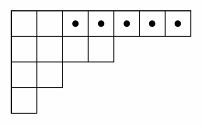
\includegraphics{./figures/L3.1}
\end{figure}

with $a_{1, 2} = 5$

\begin{ndefi}[Legs]
  Let $\l \vdash n$. For the box $b$ with coordinates $(i, j)$ in the diagram of shape $\l$, its leg, $L_b$, consists of all boxes on the same column below $b$.
  $$ L_b = \{ (i', j) \text{ a box of } \l \,|\, i' > i\} $$
\end{ndefi}

It's arm length is $l_b = |L_b|$.

\begin{figure}[!ht]
  \centering
  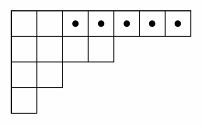
\includegraphics{./figures/L3.1}
\end{figure}

with $l_{1, 2} = 2$

Let $\l \vdash n$. It follows that, from the definitions,
$$ h_{i, j} = a_{i,j} + l_{i, j} + 1 $$

\begin{ndefi}[Hook Tableux]
  A hoot tableaux of shape $\l$ is a diagram $J$ of shape $\l$ with integer entries satisfying,
  $$ -l_{i,j} \le J_{i,j} \le a_{i,j} $$
\end{ndefi}

Thus there are $h_{i,j}$ choices for the $(i, j)$ entries in a hook tableau and so $\prod_{(i,j)\in \l} h_{i, j}$ hook tableaux of shape $\l$. We have produced a reasonable set with the size is an important player in the hook formula. This look vaugely relevant in the denominator of the hook formula.

\subsection{The Bijective Proof}


We can to rewrite the hook formula,
$$ n! = f^{\l}\prod_{(i,j) \in \l} h_{i,j} $$
A bijective proof is forming a bijection between two finite sets, so look at the size and say they are the same size, so sets are basically the same. Hence we want natural number equal natural number. Recall that there are $n!$ tableaux of shape $\l$.

So we can prove the formula by establishing a bijection,
% make this vertical
$$ \{\text{Young tableux of shape $\l$}\} \iff \{(P, J)\,|\, \text{$P$ a standard young tableau of shape $\l$ and $J$ a hook tableau of shape $\l$}\} $$
We are going to note that using pairs is useful in bijective proofs. We now have a plan. We shall show the forward direction, but not show it's a bijection.\\

\subsubsection{The Forward Direction - Standardisation Algorithm}
We want to standardise the tableau ($P$) and we can track what we are doing, i.e. tracking data $J$. We are going to describe an algorithm to a syandard youngs tableau and then track things using $J$. This gives a forward direction.\\

This process is carried out on the entries in the box of $T$, ordered from the bottom and the right. I.e,
$$ (i, j) \le (i', j') \iff j > j' \text{ or } j = j' \text{ and } i \ge i' $$

For example, consider $\l = (3, 2, 1)$ and the order,
\begin{figure}[!ht]
  \centering
  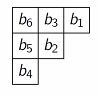
\includegraphics{./figures/L3.3}
\end{figure}

\begin{notation}
  We write $T^{\le b}$ to be the part of $T$ containing all the indicated boxes. Similarly $T^{< b}$
\end{notation}

The algorithm will construct a sequence of pairs $(T_1, J_1) = (T, 0),(T_2, J_2),\dots, (T_n, J_n) = (P,J)$ (the zero is a zero hook tableau and at the end $P$ is standard), such that $T^{\le b_k}$ is standard and $J_k$ is a hook tableau which is zero outside $J^{\le b_k}_k$. We are increasing the standardisation at each step. \\

\noindent
We need to know what we do at each step, to each $T$'s and the $J$'s. For a box $b = (i, j)$ such that $T^{< b}$ is standard while $T^{\le b}$ is not standard. Do: Consider the entries next to $b$ to the right and below, which ever is smaller (call it $b'$), swap them. Rename $b'$ as $b$ and repeat. When $T^{\le b}$ is standard, stop.\\

\noindent
How do we know this terminates? $T^{\le b}$ will eventually become standard, in the worst case when there are no further boxes to the right or down from $b$. When the process terminates, we have our next $T$.\\

\newpage
For the hook tableau $J$ which tracks the changes, we start from $J_1$ with all entries of $0$. Then if the entry in position $(i, j)$ moves to position  $(i', j')$, we change $J$ as follows. It only changes in position in column $j$ and $i$ to $i'$:
$$ (J_{\text{new}})_{h,j} = \begin{cases}
  (J_{\text{old}})_{h+1,j-1} & \text{ for $i \le h < i'$}\\
  j'-j & \text{for $h = i'$}
\end{cases} $$

So start position $(i, j)$ and end position $(i', j')$, the change to $J$ is:
\begin{figure}[!ht]
  \centering
  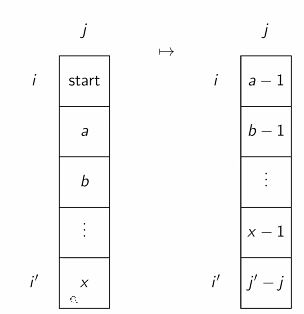
\includegraphics{./figures/L3.4}
  \caption{The Algorithm on a few rows.}
\end{figure}

Now, let's look at an example:
\begin{figure}[!ht]
  \centering
  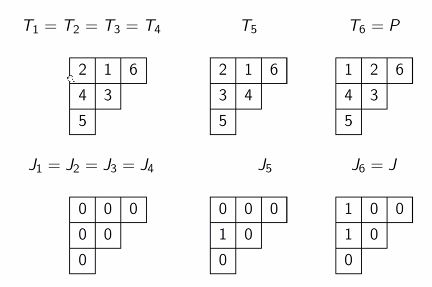
\includegraphics{./figures/L3.5}
  \caption{An example of the algorithm}
  % {Note a typo on the second row, swap on $T_6$.}
\end{figure}

We start with a non-standard tableaux $T_1$. Nothing happens for a while, we take the $6$ and then that is standard. Next, we consider $6$ and $3$, then they are again standard. Now, $6, 3$ and $1$, this is again standard. We have something to check, but these three are standard. Next, again they are disconnected and so standard. We now go to $T_5$ and we now have to do something, the $4$ violates the standardness. We now look at the right and see a $3$ and a $5$ below. $3$ is lower, so we now swap them. Now check if it's standard, but it is, so can output $T_5$. We add a just change the $(1, 2)$ zero to one in $J_5$. Now we go to the last box and look at the $2$. Is it standard? No, so move through the standard steps, we see $1$ and $3$ and so swap $1$ and $2$. Then do the same previous case in the tracking data. \footnote{ Note a typo on the second row, swap on $T_6$.}

\subsubsection{Role of Hook Length}
We must check that each $J$ is a hook tableau. Essentially, $J$ keeps track of how many places to the right and down each entry moves and this gives the constraints of a hook tableau.
From $(i, j)$ we can at most moce $a_{i,j}$ to the right, so the upper bound should be clear. And we can move at most $l_{i,j}$ places down. This gives the lower bound, which is attained in the case where everything below $(i, j)$ has it's order reversed. It should be plausible that the tracking data in the $J$'s provide enough data to go from $T$ to $P$. This is proved by setting up a map in the other direction and prove it's an inverse of the previous process. It's an algorithm which reverses the provious steps. It's a bit more technical to describe and it involves some details that means its sometimes not well behaved.

Heres how it works, $\l = (2, 1) \vdash 3$. Considering the lengths we see that $J$ has $-1 \le J_{1, 1} \le 1$ and $H_{2, 1} = J_{2,1} = 0$. There are 6 young tableux of shape $(2, 1)$, as seen above. The first two are the only standard ones. Then we can see corresponding pairs to them under the bijection,

\begin{figure}[!ht]
  \centering
  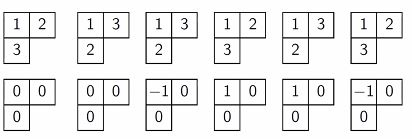
\includegraphics{./figures/L3.6}
\end{figure}
we can see the $J$'s below with tracking data and tracking data of $-1$, as we are moving things down.

\section{Links to Symmetric Group}
This lecture is an attempt to answer the question, who cares?

One answer is,\\
$$f^\l = \text{ the dimension of the irreducible representation $S^\l$ of the symmetric group $S_n$ to the partition $\l \vdash n$.}$$
Very loosely, a representation is an object on which the group acts, and an irreducible one that doesn't contain any smaller non-trivial ones. We will be looking specifically at vector spaces and we can build our actions from smaller building blocks, which are our irreducible representations.

\subsection{Group Representation}

\begin{ndefi}[Group Representations]
  Let $G$ be a finite group with idenity $e$. A (finite dimensional complex vector space) representation of $G$ is a finite dimensional complex vectorspace $V$, with an action of $G$.
\end{ndefi}

\begin{ndefi}[Group Action]
  For $g \in G$ and $v\in V$, we have $gv \in V$ satisfying,
  \begin{itemize}
    \item $ev = v$ (identity acts as identity)
    \item $(gh)v = g(hv)$ (compatibility of the action with group multiplication)
    \item $g(\a v + \b w) = \a (gv) + \b (gw)$ (compatibility of the action with the vector space structure)
  \end{itemize}
  for all $g, h \in G$, $v, w \in V$ and $\a, \b \in \C$.
\end{ndefi}

\begin{ndefi}[Subrepresentation]
  A vector subspace that preserved the group action
\end{ndefi}

\begin{ndefi}[Irreducible]
  A representation is irreducible if it doesn't have any non-trivial subrepresentation.
\end{ndefi}

Let's look at some examples:
\begin{itemize}
  \item The \textit{trivial} representation. Let $V = \C$ and let $\pi v = v$ for all $\pi \in S_n$ and $v \in \C$
  \item The \text{sign} representation: let $V = \C$ and let $\pi v = \sgn(\pi)v$ for all $\pi \in S_n$ and all $v \in \C$.
\end{itemize}

\begin{remark}
  You can always write a permutation as a composite of transposition (2-cycles), not uniquely, but if you see an even number of transpositions you will always get an even number, same for odd. It's not invariant, but the sign defined as $+1$ if it's even, but $-1$ if it's odd and it's invariant.\\
  Also the sign of a product is the product of the signs.
\end{remark}
These are the only one dimensional representations.

\begin{itemize}
  \item The \textit{natural} representation: let $V = \C$ and let $S_n$ act by permuting the $n$ standard basis vectors. So,
  $$ \pi\left(\sum_{i=1}^n {\a_ie_i}\right) = \sum_{i=1}^n {\a_ie_{\pi(i)}} $$
  \item The regular representation: let $V$ be an $n!$ dimensional complex vector space with basis $\{e_{\sigma} = \s \in S_n\}$. The action is determined by the action od the group on itself, $\pi(e_\s) = e_{\pi \s}$.
\end{itemize}

The first two of these examples are irreducible, the trivial is always irreducible.

The natural representation is not irreducible, its a sum of two irreducible pieces.
The regular representation is also very much not irreducible. Every single irreducible representation lives in the regular representation.

\newpage
\subsection{Tabloids}
We want to start with a partition and construct an irreducible representation of the symmetric group.

\begin{ndefi}[Row Equivilent]
  We say that two tableaux of shape $\l$ are row equivalent if the corresponding rows contain the same elements.
\end{ndefi}

\begin{figure}[!ht]
  \centering
  \begin{ytableau}
         1 & 2 & 3 \\
         4 & \none & \none
  \end{ytableau}\hspace{20pt}
  \begin{ytableau}
         3 & 4 & 1 \\
         1 & \none & \none
  \end{ytableau}
\end{figure}


\begin{ndefi}[Tabloid]
  The tabloid of shape $\l$ is an equivilence class of shale $\l$ under row equivilence. We denote it as $\mathbf{t}$
\end{ndefi}

We shall write a tabloid as,
\begin{figure}[!ht]
\centering
% notabloids
\ytableausetup{tabloids,centertableaux}
\ytableaushort{123,4}
% 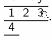
\includegraphics{./figures/L4.2}
\end{figure}

\subsection{Constructing $S^\l$}
Firstly start with a young tableau $t$ of shape $\l$.\\
Define an associated column group $C_t$.\\
Define $\kappa_t$ as a signed sum over the column group, $C_t$.\\
Define $e_t = \kappa_t \mathbf{t}$ a linear combination of tabloids of shape $\l$.\\
Then $S^\l$ is thr set of complex linear combination of $e_t$ where $t$ is the tableau of shape $\l$.\\

\subsubsection{Details}
Let $t$ be a young tableau of hape $\l \vdash n$ and let $C_i$ be the subgroup of $S_n$ consisting of perms of the entries of the column $i$. Then $C_t$ is the associated column group,
$$ C_t = C_1 \times C_2 \times \dots \times C_k $$
For example, if t is,
\begin{figure}[!ht]
  \centering
  \ytableausetup{centertableaux}
  \ytableaushort{125,34} % this may be incorrect
\end{figure}\footnote{Is this correct?}
we can say,
$$ C_t = \{1, (1 3), (2 4), (1 3)(2 4)\}  $$
Then,
$$ \kappa_t = \sum_{\pi \in C_t}{\sgn (\pi)\pi} $$
\newpage
This is a linear combination of elements of th symmetric group. For example, its just,
$$ \kappa_t = 1 - (1 3) - (2 4) + (1 3)(2 4)  $$
and now we get to the last step,
$$ e_t = \kappa_t \mathbf{t} $$
\begin{remark}
  $e_t$ is called the polytabloid associated to the tabloid $\mathbf{t}$.
\end{remark}

\begin{remark}
   $\kappa_t$ is the signed sum over the column group. It's a linear combinations of permutations. This lives in the group algebra, this is where we take the elements and declare them a basis of a complex vector space, then we have a multiplication. \\
   Then the $e_t$ is an element of a representation (vectors), which is a complex vector space, which has an action on the group. These are also a spanning set of the representation of the partition. If we let $t$ be standard, then we get a basis.
\end{remark}

For example,

\begin{figure}[!ht]
\centering
\ytableausetup{centertableaux}
\ytableaushort{125,34}\hspace{10pt} - \hspace{10pt} \ytableaushort{325,14}\hspace{10pt} - \hspace{10pt}\ytableaushort{145,32}\hspace{10pt} + \hspace{10pt}\ytableaushort{345,12}
\end{figure}

\begin{ex}
  Checking the details of the examples is one of the exercises
\end{ex}

\begin{itemize}
  \item $S^{(n)}$ is just the trivial representation.
  \item $S^{(1,1,\dots,1)}$ is the sign representation.
  \item $S^{(n-1,1)}$ is an $n-1$ dimensional representation and the natural representation is a direct sum of this and the trivial representation.
\end{itemize}

\begin{nthm}[]
  The set,
  $$ \{e_t \,|\, t \text{ is a stanrd tableau of a shape } \l\} $$
  is a basis for $S^\l$.
\end{nthm}
\begin{proof}
  Ommited
\end{proof}

\begin{ncor}
  $$ \dim(S^{\l}) = f^{\l} $$
\end{ncor}
\begin{proof}
   Trivial
\end{proof}

Example of a basis, let $\l = (2, 1) \vdash 3$. We have two standard tableaux, say $t$ and $t'$ of shape $\l$:
%insert theorem
Then $e_t$ is,
\begin{figure}[!ht]
\centering
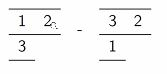
\includegraphics{./figures/L4.4}
\end{figure}
Then $e_{t'}$ is,
\begin{figure}[!ht]
\centering
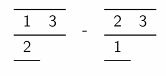
\includegraphics{./figures/L4.5}
\end{figure}
and $S^\l$ is the $2$-dimensional representation of $S_3$ with basis, $\{e_t, e_{t'}\}$

\begin{remark}
 Every finite dimensional representation is a direct sum of irriductible representations.
\end{remark}

\subsection{A Run around Representation Theory.}
\begin{itemize}
  \item The number of irreducible representation of a finite group $G$ is equal to the number of conjuagcy classes of the group.
  \item So for $S_n$, the number of irriductible representations is equal to the number o partitions.
  \item For a partition of $\l$, the representation $S^\l$ is constructed above and irriducible.
  \item And the $S^\l$ are different so we have a complete list of irriducible representations.
\end{itemize}

\begin{itemize}
  \item For a finite group $G$,
  $$ \sum_{V} (\dim V)^2 = |G| $$
  where the sum is over all the irriducible representations.
  \item This follows from the fact that the regular representation contains each irriducible and the number of times each one apparears is equal to its dimension.
  \item So for $S_n$, this gives,
  $$ \sum_{\l \vdash n} (f^\l)^2 = n! $$
\end{itemize}

There is a bijection,
$$ \text{partition $\l \vdash n$} \longleftrightarrow \text{$S^\l$ irriducible representation of $S_n$} $$
$S^\l$ has a basis described in terms of the standard young tableaux of shape $\l$ and so dimension $f^\l$.\\

\newpage
\textbf{Further Reading:}\\
\begin{itemize}
  \item Equivariant Algebraic Topology (Topology and group actions / representations)
  \item Tree Representation of the Symmetric Group
  \item Modular Representation Theory.
  \item Skew Tableaux.
  \item Hyperoctohedral Groups. (Wreath product)
  \item Splitting Field.
\end{itemize}

\begin{remark}
  A transpose of a young tableaux is the tensor product of it with the sign of permutations. 
\end{remark}

\end{document}
